\documentclass{extbook}[14pt]
\usepackage{multicol, enumerate, enumitem, hyperref, color, soul, setspace, parskip, fancyhdr, amssymb, amsthm, amsmath, latexsym, units, mathtools}
\everymath{\displaystyle}
\usepackage[headsep=0.5cm,headheight=0cm, left=1 in,right= 1 in,top= 1 in,bottom= 1 in]{geometry}
\usepackage{dashrule}  % Package to use the command below to create lines between items
\newcommand{\litem}[1]{\item #1

\rule{\textwidth}{0.4pt}}
\pagestyle{fancy}
\lhead{}
\chead{Answer Key for Module6 Version A}
\rhead{}
\lfoot{2107-1615}
\cfoot{}
\rfoot{test}
\begin{document}
\textbf{This key should allow you to understand why you choose the option you did (beyond just getting a question right or wrong). \href{https://xronos.clas.ufl.edu/mac1105spring2020/courseDescriptionAndMisc/Exams/LearningFromResults}{More instructions on how to use this key can be found here}.}

\textbf{If you have a suggestion to make the keys better, \href{https://forms.gle/CZkbZmPbC9XALEE88}{please fill out the short survey here}.}

\textit{Note: This key is auto-generated and may contain issues and/or errors. The keys are reviewed after each exam to ensure grading is done accurately. If there are issues (like duplicate options), they are noted in the offline gradebook. The keys are a work-in-progress to give students as many resources to improve as possible.}

\rule{\textwidth}{0.4pt}

\begin{enumerate}\litem{
Construct the lowest-degree polynomial given the zeros below. Then, choose the intervals that contain the coefficients of the polynomial in the form $x^3+bx^2+cx+d$.
\[ 5 + 4 i \text{ and } -4 \]The solution is \( x^{3} -6 x^{2} +x + 164 \), which is option B.\begin{enumerate}[label=\Alph*.]
\item \( b \in [-2.3, 4.4], c \in [-1.6, -0.93], \text{ and } d \in [-21.5, -18] \)

$x^{3} + x^{2} -x -20$, which corresponds to multiplying out $(x -5)(x + 4)$.
\item \( b \in [-8.4, -5.6], c \in [0.11, 1.85], \text{ and } d \in [163.6, 167.2] \)

* $x^{3} -6 x^{2} +x + 164$, which is the correct option.
\item \( b \in [3, 9.5], c \in [0.11, 1.85], \text{ and } d \in [-165.4, -158.5] \)

$x^{3} +6 x^{2} +x -164$, which corresponds to multiplying out $(x-(5 + 4 i))(x-(5 - 4 i))(x -4)$.
\item \( b \in [-2.3, 4.4], c \in [-0.84, 0.88], \text{ and } d \in [-17.4, -12] \)

$x^{3} + x^{2} +0 x -16$, which corresponds to multiplying out $(x -4)(x + 4)$.
\item \( \text{None of the above.} \)

This corresponds to making an unanticipated error or not understanding how to use nonreal complex numbers to create the lowest-degree polynomial. If you chose this and are not sure what you did wrong, please contact the coordinator for help.
\end{enumerate}

\textbf{General Comment:} Remember that the conjugate of $a+bi$ is $a-bi$. Since these zeros always come in pairs, we need to multiply out $(x-(5 + 4 i))(x-(5 - 4 i))(x-(-4))$.
}
\litem{
Construct the lowest-degree polynomial given the zeros below. Then, choose the intervals that contain the coefficients of the polynomial in the form $ax^3+bx^2+cx+d$.
\[ \frac{-1}{2}, \frac{-1}{4}, \text{ and } \frac{7}{5} \]The solution is \( 40x^{3} -26 x^{2} -37 x -7 \), which is option E.\begin{enumerate}[label=\Alph*.]
\item \( a \in [35, 42], b \in [-88, -76], c \in [47, 56], \text{ and } d \in [-8, -2] \)

$40x^{3} -86 x^{2} +47 x -7$, which corresponds to multiplying out $(2x -1)(4x -1)(5x -7)$.
\item \( a \in [35, 42], b \in [-66, -63], c \in [4, 12], \text{ and } d \in [3, 13] \)

$40x^{3} -66 x^{2} +9 x + 7$, which corresponds to multiplying out $(2x -1)(4x + 1)(5x -7)$.
\item \( a \in [35, 42], b \in [20, 30], c \in [-38, -35], \text{ and } d \in [3, 13] \)

$40x^{3} +26 x^{2} -37 x + 7$, which corresponds to multiplying out $(2x -1)(4x -1)(5x + 7)$.
\item \( a \in [35, 42], b \in [-29, -24], c \in [-38, -35], \text{ and } d \in [3, 13] \)

$40x^{3} -26 x^{2} -37 x + 7$, which corresponds to multiplying everything correctly except the constant term.
\item \( a \in [35, 42], b \in [-29, -24], c \in [-38, -35], \text{ and } d \in [-8, -2] \)

* $40x^{3} -26 x^{2} -37 x -7$, which is the correct option.
\end{enumerate}

\textbf{General Comment:} To construct the lowest-degree polynomial, you want to multiply out $(2x + 1)(4x + 1)(5x -7)$
}
\litem{
Describe the zero behavior of the zero $x = 8$ of the polynomial below.
\[ f(x) = -7(x - 2)^{10}(x + 2)^{6}(x + 8)^{11}(x - 8)^{6} \]The solution is the graph below, which is option B.
\begin{center}
    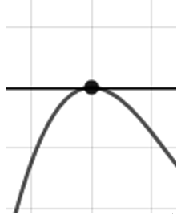
\includegraphics[width=0.3\textwidth]{../Figures/polyZeroBehaviorBA.png}
\end{center}\begin{enumerate}[label=\Alph*.]
\begin{multicols}{2}
\item 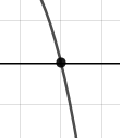
\includegraphics[width = 0.3\textwidth]{../Figures/polyZeroBehaviorAA.png}
\item 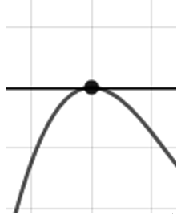
\includegraphics[width = 0.3\textwidth]{../Figures/polyZeroBehaviorBA.png}
\item 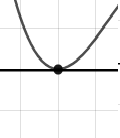
\includegraphics[width = 0.3\textwidth]{../Figures/polyZeroBehaviorCA.png}
\item 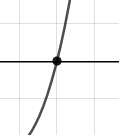
\includegraphics[width = 0.3\textwidth]{../Figures/polyZeroBehaviorDA.png}
\end{multicols}\item None of the above.\end{enumerate}
\textbf{General Comment:} You will need to sketch the entire graph, then zoom in on the zero the question asks about.
}
\litem{
Describe the zero behavior of the zero $x = 8$ of the polynomial below.
\[ f(x) = -9(x - 5)^{12}(x + 5)^{9}(x + 8)^{10}(x - 8)^{7} \]The solution is the graph below, which is option A.
\begin{center}
    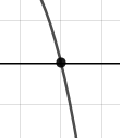
\includegraphics[width=0.3\textwidth]{../Figures/polyZeroBehaviorCopyAA.png}
\end{center}\begin{enumerate}[label=\Alph*.]
\begin{multicols}{2}
\item 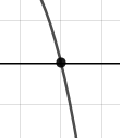
\includegraphics[width = 0.3\textwidth]{../Figures/polyZeroBehaviorCopyAA.png}
\item 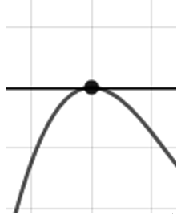
\includegraphics[width = 0.3\textwidth]{../Figures/polyZeroBehaviorCopyBA.png}
\item 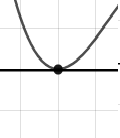
\includegraphics[width = 0.3\textwidth]{../Figures/polyZeroBehaviorCopyCA.png}
\item 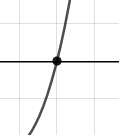
\includegraphics[width = 0.3\textwidth]{../Figures/polyZeroBehaviorCopyDA.png}
\end{multicols}\item None of the above.\end{enumerate}
\textbf{General Comment:} You will need to sketch the entire graph, then zoom in on the zero the question asks about.
}
\litem{
Which of the following equations \textit{could} be of the graph presented below?

\begin{center}
    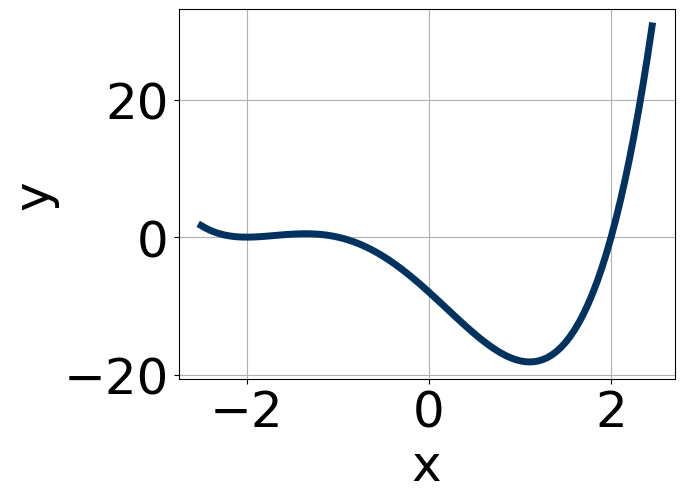
\includegraphics[width=0.5\textwidth]{../Figures/polyGraphToFunctionCopyA.png}
\end{center}


The solution is \( -17x^{4} (x + 4)^{4} (x + 1)^{6} \), which is option C.\begin{enumerate}[label=\Alph*.]
\item \( -8x^{7} (x + 4)^{4} (x + 1)^{11} \)

The factors $x$ and $(x + 1)$ should both have even powers.
\item \( -14x^{10} (x + 4)^{8} (x + 1)^{9} \)

The factor $(x + 1)$ should have an even power.
\item \( -17x^{4} (x + 4)^{4} (x + 1)^{6} \)

* This is the correct option.
\item \( 14x^{10} (x + 4)^{6} (x + 1)^{9} \)

The factor $(x + 1)$ should have an even power and the leading coefficient should be the opposite sign.
\item \( 13x^{8} (x + 4)^{10} (x + 1)^{10} \)

This corresponds to the leading coefficient being the opposite value than it should be.
\end{enumerate}

\textbf{General Comment:} General Comments: Draw the x-axis to determine which zeros are touching (and so have even multiplicity) or cross (and have odd multiplicity).
}
\litem{
Describe the end behavior of the polynomial below.
\[ f(x) = 5(x + 3)^{3}(x - 3)^{8}(x + 7)^{3}(x - 7)^{5} \]The solution is the graph below, which is option D.
\begin{center}
    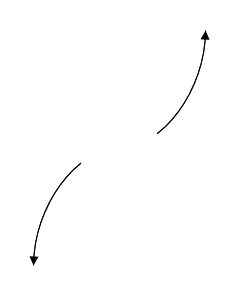
\includegraphics[width=0.3\textwidth]{../Figures/polyEndBehaviorDA.png}
\end{center}\begin{enumerate}[label=\Alph*.]
\begin{multicols}{2}
\item 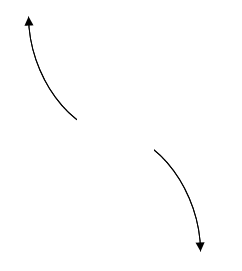
\includegraphics[width = 0.3\textwidth]{../Figures/polyEndBehaviorAA.png}
\item 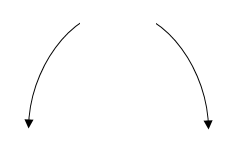
\includegraphics[width = 0.3\textwidth]{../Figures/polyEndBehaviorBA.png}
\item 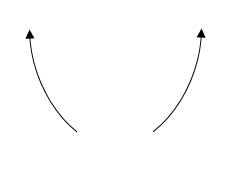
\includegraphics[width = 0.3\textwidth]{../Figures/polyEndBehaviorCA.png}
\item 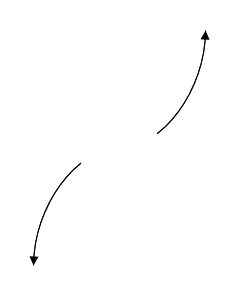
\includegraphics[width = 0.3\textwidth]{../Figures/polyEndBehaviorDA.png}
\end{multicols}\item None of the above.\end{enumerate}
\textbf{General Comment:} Remember that end behavior is determined by the leading coefficient AND whether the \textbf{sum} of the multiplicities is positive or negative.
}
\litem{
Construct the lowest-degree polynomial given the zeros below. Then, choose the intervals that contain the coefficients of the polynomial in the form $x^3+bx^2+cx+d$.
\[ -4 - 5 i \text{ and } 4 \]The solution is \( x^{3} +4 x^{2} +9 x -164 \), which is option C.\begin{enumerate}[label=\Alph*.]
\item \( b \in [-8, -3], c \in [8.79, 9.4], \text{ and } d \in [160, 168] \)

$x^{3} -4 x^{2} +9 x + 164$, which corresponds to multiplying out $(x-(-4 - 5 i))(x-(-4 + 5 i))(x + 4)$.
\item \( b \in [-1, 2], c \in [0.48, 1.62], \text{ and } d \in [-24, -18] \)

$x^{3} + x^{2} +x -20$, which corresponds to multiplying out $(x + 5)(x -4)$.
\item \( b \in [2, 5], c \in [8.79, 9.4], \text{ and } d \in [-165, -163] \)

* $x^{3} +4 x^{2} +9 x -164$, which is the correct option.
\item \( b \in [-1, 2], c \in [-0.13, 0.06], \text{ and } d \in [-18, -14] \)

$x^{3} + x^{2} +0 x -16$, which corresponds to multiplying out $(x + 4)(x -4)$.
\item \( \text{None of the above.} \)

This corresponds to making an unanticipated error or not understanding how to use nonreal complex numbers to create the lowest-degree polynomial. If you chose this and are not sure what you did wrong, please contact the coordinator for help.
\end{enumerate}

\textbf{General Comment:} Remember that the conjugate of $a+bi$ is $a-bi$. Since these zeros always come in pairs, we need to multiply out $(x-(-4 - 5 i))(x-(-4 + 5 i))(x-(4))$.
}
\litem{
Construct the lowest-degree polynomial given the zeros below. Then, choose the intervals that contain the coefficients of the polynomial in the form $ax^3+bx^2+cx+d$.
\[ -7, \frac{-3}{2}, \text{ and } \frac{-5}{3} \]The solution is \( 6x^{3} +61 x^{2} +148 x + 105 \), which is option C.\begin{enumerate}[label=\Alph*.]
\item \( a \in [0, 7], b \in [-44, -36], c \in [-26, -17], \text{ and } d \in [101, 112] \)

$6x^{3} -41 x^{2} -22 x + 105$, which corresponds to multiplying out $(x -7)(2x -3)(3x + 5)$.
\item \( a \in [0, 7], b \in [59, 62], c \in [138, 153], \text{ and } d \in [-109, -103] \)

$6x^{3} +61 x^{2} +148 x -105$, which corresponds to multiplying everything correctly except the constant term.
\item \( a \in [0, 7], b \in [59, 62], c \in [138, 153], \text{ and } d \in [101, 112] \)

* $6x^{3} +61 x^{2} +148 x + 105$, which is the correct option.
\item \( a \in [0, 7], b \in [-26, -18], c \in [-119, -111], \text{ and } d \in [-109, -103] \)

$6x^{3} -23 x^{2} -118 x -105$, which corresponds to multiplying out $(x -7)(2x + 3)(3x + 5)$.
\item \( a \in [0, 7], b \in [-65, -60], c \in [138, 153], \text{ and } d \in [-109, -103] \)

$6x^{3} -61 x^{2} +148 x -105$, which corresponds to multiplying out $(x -7)(2x -3)(3x -5)$.
\end{enumerate}

\textbf{General Comment:} To construct the lowest-degree polynomial, you want to multiply out $(x + 7)(2x + 3)(3x + 5)$
}
\litem{
Describe the end behavior of the polynomial below.
\[ f(x) = -4(x - 5)^{3}(x + 5)^{4}(x + 6)^{3}(x - 6)^{3} \]The solution is the graph below, which is option A.
\begin{center}
    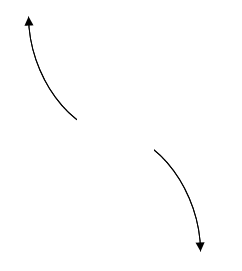
\includegraphics[width=0.3\textwidth]{../Figures/polyEndBehaviorCopyAA.png}
\end{center}\begin{enumerate}[label=\Alph*.]
\begin{multicols}{2}
\item 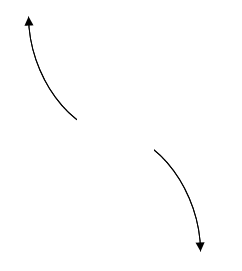
\includegraphics[width = 0.3\textwidth]{../Figures/polyEndBehaviorCopyAA.png}
\item 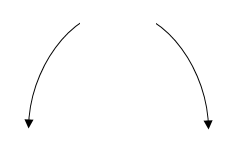
\includegraphics[width = 0.3\textwidth]{../Figures/polyEndBehaviorCopyBA.png}
\item 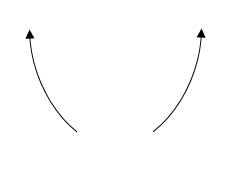
\includegraphics[width = 0.3\textwidth]{../Figures/polyEndBehaviorCopyCA.png}
\item 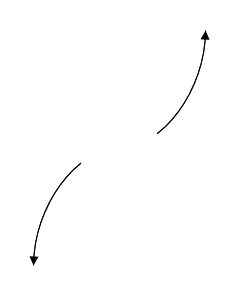
\includegraphics[width = 0.3\textwidth]{../Figures/polyEndBehaviorCopyDA.png}
\end{multicols}\item None of the above.\end{enumerate}
\textbf{General Comment:} Remember that end behavior is determined by the leading coefficient AND whether the \textbf{sum} of the multiplicities is positive or negative.
}
\litem{
Which of the following equations \textit{could} be of the graph presented below?

\begin{center}
    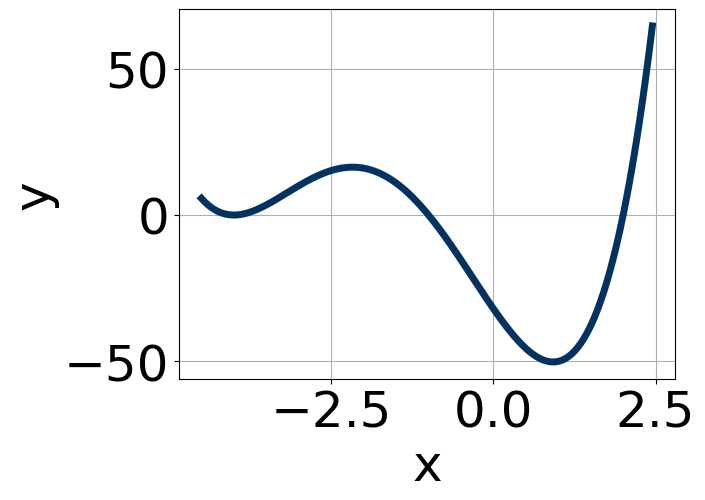
\includegraphics[width=0.5\textwidth]{../Figures/polyGraphToFunctionA.png}
\end{center}


The solution is \( -12x^{9} (x + 1)^{8} (x - 1)^{5} \), which is option C.\begin{enumerate}[label=\Alph*.]
\item \( 10x^{11} (x + 1)^{4} (x - 1)^{5} \)

This corresponds to the leading coefficient being the opposite value than it should be.
\item \( -8x^{7} (x + 1)^{8} (x - 1)^{10} \)

The factor $(x - 1)$ should have an odd power.
\item \( -12x^{9} (x + 1)^{8} (x - 1)^{5} \)

* This is the correct option.
\item \( 3x^{10} (x + 1)^{4} (x - 1)^{11} \)

The factor $x$ should have an odd power and the leading coefficient should be the opposite sign.
\item \( -10x^{9} (x + 1)^{9} (x - 1)^{10} \)

The factor $-1$ should have an even power and the factor $1$ should have an odd power.
\end{enumerate}

\textbf{General Comment:} General Comments: Draw the x-axis to determine which zeros are touching (and so have even multiplicity) or cross (and have odd multiplicity).
}
\end{enumerate}

\end{document}